\documentclass[11pt]{beamer}
\usetheme{Warsaw}
\usepackage[utf8]{inputenc}
\usepackage[francais]{babel}
\usepackage[T1]{fontenc}
\usepackage{amsmath}
\usepackage{amsfonts}
\usepackage{amssymb}
\usepackage{graphicx}
\author{Amghar  Mohamed}
\title{Modèle linièare mixtes }
\institute{Enseignant : Mr Salmon Joseph} 
\titlegraphic{ \includegraphics[scale=0.1]{t.JPG} }
%\transparent
\date{08/11/2020} 
\AtBeginSubsection[]
{ \begin{frame}
\frametitle{Tables des matières}
\tableofcontents[setionstyle=show/hide,subsubsectionstyle=show/hide, subsectionstyle=show/shaded]
\end{frame}
}
\begin{document}

\begin{frame}
\titlepage
\end{frame}

\begin{frame}
\frametitle{Tables des matières}
\tableofcontents[setionstyle=show,subsubsectionstyle=show, subsectionstyle=show]
\end{frame}

\section{Introduction}
\begin{center}
Présentation des données:\\
    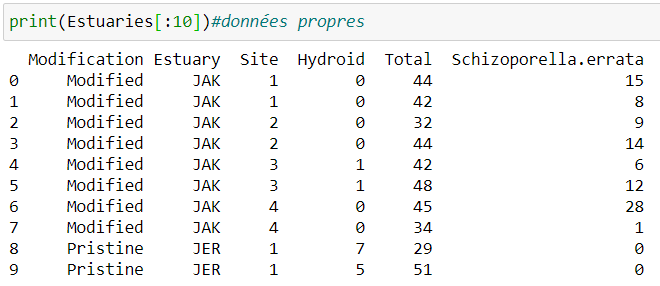
\includegraphics[scale=0.65]{headdonn.PNG}
\end{center}
\subsection{modèle linièare mixte} 
\subsubsection{ Définitions }
\begin{frame}
\begin{block}{Définition}
\textbf{modèle linièare mixte}\\
 Un modèle linéaire mixte est un modèle pour lequel le modèle comprend à la fois des effets fixes et des
effets aléatoires. Les MLM incluent des variables à effets fixes et aléatoires. Le mélange entre les deux est à
l'origine du nom. Les effets fixes décrivent les relations entre les covariables et la variable dépendante pour
une population entière, les effets aléatoires sont spécifiques à l'échantillon.\\
En d'autres termes, un effet aléatoire est un effet dont nous ne voulons pas généraliser les propriétés (les
modalités ont été choisies de manière aléatoire dans quelque chose de plus grand) et un effet fixe est un
effet dont on veut généraliser les propriétés. Il s'agit de la variable manipulée dont nous avons choisi les
niveaux spécifiques.
\end{block}
\end{frame}

\begin{frame}
\begin{block}{Hypothèse: }
Les modèles mixtes font des hypothèses importantes:\\
1. (y|x) sont i.i.d et suit loi normale\\
2. V(y|x) est constante\\
3. y s'écrit sous forme linéaire en fonction de x et z(l'effet aléatoire) .\\
4. y est indépendant de z\\
5. z suit loi normale.\\
\end{block}
\end{frame}
\subsubsection{Interprétation: }
\begin{center}
    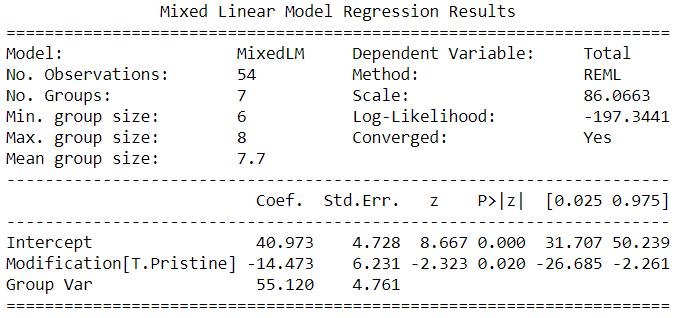
\includegraphics[scale=0.65]{modele1.PNG}
\end{center}

comparaison des deux modèles:
\begin{center}
    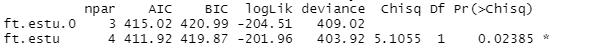
\includegraphics[scale=0.65]{Comparaisonmmod.PNG}
\end{center}



\section{modèle linéaire mixte 2:}
\subsection{}
\begin{frame}
\begin{block}{Hypothèse: }
Deux facteurs sont croisés lorsque chaque catégorie (niveau) d'un facteur coexiste dans la conception avec chaque catégorie de l'autre facteur. En d'autres termes, il y a au moins une observation dans chaque combinaison de catégories pour les deux facteurs.
\end{block}
\end{frame}
\begin{frame}
\begin{block}{Hypothèse: }
Les mêmes hypothèses pour les modèles à effets mixte 2:\\
1. (y|x) sont i.i.d et suit loi normale\\
2. V(y|x) est constante\\
3. y s'écrit sous forme linéaire en fonction de x et z(l'effet aléatoire) .\\
4. y est indépendant de z\\
5. z suit loi normale.\\
\end{block}
\end{frame}
\begin{frame}
\begin{center}
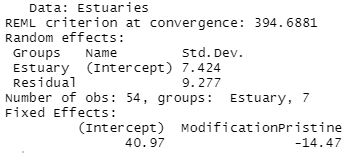
\includegraphics[scale=0.75]{ajustmod1.PNG}
\end{center}
\end{frame}
\begin{frame}
\begin{center}
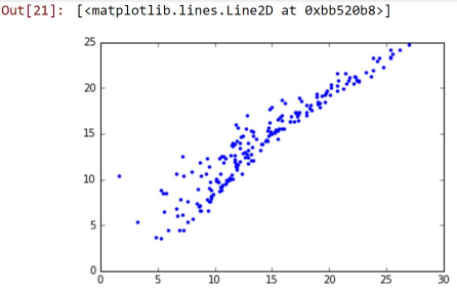
\includegraphics[scale=0.65]{plotdon.PNG}
\end{center}
\end{frame}
\begin{frame}
\begin{center}
\textbf{bootstrap paramétrique:}\\
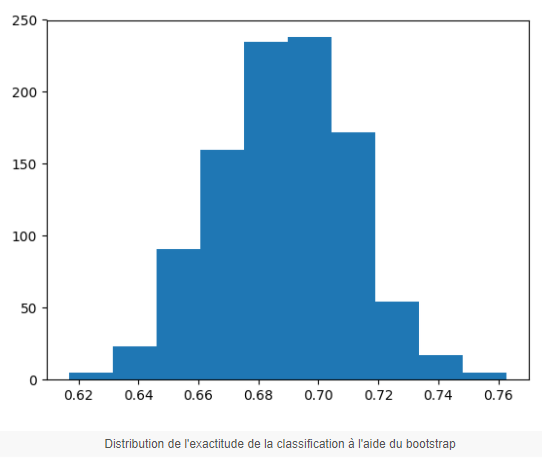
\includegraphics[scale=0.65]{distribdonbootstrap.PNG}
\end{center}
\end{frame}



\begin{frame}[plain]{}
\begin{center}
    \LARGE\color{blue}
\textbf{MERCI!}
\end{center}
\end{frame}


\end{document}